\setcounter{chapter}{17}

\chapter{Credibility and Bonus-Malus}


{\small \textit{Chapter Preview}. This chapter introduces regression
applications of pricing in credibility and bonus-malus experience
rating systems. Experience rating systems are formal methods for
including claims experience into renewal premiums of short-term
contracts, such automobile, health and workers compensation. This
chapter provides brief introductions to credibility and bonus-malus,
emphasizing their relationship with regression methods.}

\section{Risk Classification and Experience Rating}\index{actuarial \& financial terms and concepts!risk classification}
\index{actuarial \& financial terms and concepts!experience
rating}\index{actuarial \& financial terms and concepts!merit
rating}


Risk classification is a key ingredient of insurance pricing.
Insurers sell coverage at prices that are sufficient to cover
anticipated claims, administrative expenses and an expected profit
to compensate for the cost of capital necessary to support the sale
of the coverage. In many countries and lines of business, the
insurance market is mature and highly competitive. This strong
competition induces insurers to classify risks they underwrite in
order to receive fair premiums for the risk undertaken. This
classification is based on \emph{known} characteristics of the
insured, the person or firm seeking the insurance coverage.

\marginparjed{Insurers classify risks based on known characteristics
of the insured, the person or firm seeking coverage.}

For example, suppose that you are working for a company that insures
small businesses for time lost due to employees injured on the job.
Consider pricing this insurance product for two businesses that are
identical with respect to number of employees, location, age and
gender distribution and so forth, except that one company is a
management consulting firm and the other is a construction firm.
Based on experience, you expect the management consulting firm to
have a lower claims level than the construction firm and you need to
price accordingly. If you do not, another insurance company will
offer a lower insurance price to the consulting firm and take this
potential customer away, leaving your company with only the more
costly construction firm business.

Competition among insurers leads to charging premiums according to
observable characteristics, known as \textit{risk classification}.
In the context of regression modeling, we can think of this as
modeling the claims distributions in terms of explanatory variables.

Many pricing situations are based on a relationship between the
insurer and the insured that develops over time. These relationships
allow insurers to base prices on \emph{unobservable} characteristics
of the insured by taking into account the prior claims experience of
the insured. Modifying premiums with claims history is known as
\emph{experience rating}, also sometimes referred to as
\textit{merit rating}.

Experience rating methods are either applied retrospectively or
prospectively. With retrospective methods, a ``refund'' of a portion
of the premium is provided to the insured in the event of favorable
(to the insurer) experience. Retrospective premiums are common in
life insurance arrangements (where insureds earned ``dividends'' in
the U.S. and ``bonuses'' in the U.K.). In property and casualty
insurance prospective methods are more common, where favorable
insured experience is ``rewarded'' through a lower renewal premium.

In this chapter, we discuss two prospective methods that are
well-suited for regression modeling, credibility and bonus-malus.
Bonus-malus methods are used extensively in Asia and Europe,
although almost exclusively with automobile insurance. As we will
see in Section \ref{S18:Bonus-Malus}, the idea is to use claims
experience to modify the classification of an insured. Credibility
methods, introduced in Section \ref{S18:Cred}, are more broadly
applied in terms of lines of business and geography.


\section{Credibility}\label{S18:Cred}\index{actuarial \& financial terms and concepts!credibility}

Credibility is a technique for pricing insurance coverages that is
widely used by health, group term life and property and casualty
actuaries. In the United States, the standards are described under
the Actuarial Standard of Practice Number 25 published by the
Actuarial Standards Board of the American Academy of Actuaries (web
site: http://www.actuary.org/). Further, several insurance laws and
regulation require the use of credibility.

The theory of credibility has been called a ``cornerstone'' of the
field of actuarial science (Hickman and Heacox, 1999). The basic
idea is to use claims experience and additional information to
develop a pricing formula, such as through the relation
\begin{equation}\label{E18:Cred}
New~Premium =  \zeta \times Claims~Experience + (1 - \zeta)  \times
Old~Premium.
\end{equation}
Here, $\zeta$ (the Greek letter ``zeta'') is known as the
``credibility factor;'' values generally lie between zero and one.
The case $\zeta=1$ is known as ``full credibility,'' where claims
experience is used solely to determine the premium. The case
$\zeta=0$  can be thought of as ``no credibility,'' where claims
experience is ignored and external information is used as the sole
basis for pricing.

To keep this chapter self-contained, we begin by introducing some
basic credibility concepts. Section \ref{S18:LimFCred} reviews
classic concepts of credibility, including when to use it and linear
pricing formulas. Section \ref{S18:GreatestAccCred} describes the
modern version of credibility by introducing a formal probabilistic
model that can be used for updating insurance prices. Section
\ref{S18:CredRegression} discusses the link with regression
modeling.


\subsection{Limited Fluctuation Credibility}\label{S18:LimFCred}

Credibility has a long history in actuarial science, with
fundamental contributions dating back to Mowbray (1914).
Subsequently, Whitney (1918) introduced the intuitively appealing
concept of using a weighted average of (1) claims from the risk
class and (2) claims over all risk classes to predict future
expected claims.


\subsubsection*{Standards for Full Credibility}

The title of Mowbray's paper was ``How extensive a payroll exposure
is necessary to give a dependable pure premium?'' It is still the
first question that an analyst needs to confront: when do I need to
use credibility estimators? To get a better handle on this question,
consider the following situation.

\linejed

\textbf{Example: Dental Costs.} Suppose that you are pricing dental
insurance coverage for a small employer. For males aged 18-25, the
employer provides the following experience:
\begin{center}\scalefont{0.90}
\begin{tabular}{lrrr}
  \hline
  Year & 2007 & 2008 & 2009 \\
  Number & 8 & 12 & 10 \\
  Average Dental Cost & 500 & 400 & 900 \\
  \hline
\end{tabular}\scalefont{1.1111}\end{center}

\noindent The ``manual rate,'' available from a tabulation of a much
larger set of data, is \$700 per employee. Ignoring inflation and
expenses, what would you use to anticipate dental costs in 2010? The
manual rate? The average of the available data? Or some combination?

\index{actuarial \& financial terms and concepts!manual rate}

\linejed

Mowbray wanted to distinguish between situations when (1) large
employers with substantial information could use their own
experience and (2) small employers with limited experience would use
external sources, so-called ``manual rates.'' In statistical
terminology, we can think about forming an estimator from an
employer's experience of the true mean costs. We are asking whether
the distribution of the estimator is sufficiently close to the mean
to be reliable. Of course, ``sufficiently close'' is the tricky
part, so let us look at a more concrete situation.

The simplest set-up is to assume that you have claims $y_1, \ldots,
y_n$ that are identically and independently distributed (i.i.d.)
with mean $\mu$ and variance $\sigma^2$. As a standard for full
credibility, we could require that $n$ be large enough so that

\begin{equation}\label{E18:FullCredib}
\Pr ( (1-r) \mu \leq \bar{y} \leq (1+r) \mu) \geq p,
\end{equation}
where $r$ and $p$ are given constants. For example, if $r=0.05$ and
$p=0.9$, then we wish to have at least 90\% chance of being within
5\% of the mean.

Using normal approximations, it is straight-forward to show that
sufficient for equation (\ref{E18:FullCredib}) is

\begin{equation}\label{E18:FullCredib1}
n \geq \left(\frac{\Phi^{-1}(\frac{p+1}{2}) \sigma}{r \mu} \right)^2
.
\end{equation}
We define $n_F$, the number of observations required for full
credibility, to be the smallest value of $n$ that satisfies equation
(\ref{E18:FullCredib1}).

\linejed

\textbf{Example: Dental Costs - Continued.} From the table, average
costs are $\bar{y} = \left( 500 \times 8 + 400 \times 12 + 900
\times 10 \right)/30 = 593.33.$ Suppose that we have available an
estimate of the standard deviation $\sigma \approx \widehat{\sigma}=
200.$ Using $p=0.90$, the 90th percentile of the normal distribution
is $\Phi^{-1}(.95) = 1.645$. With $r=0.05$, the approximate sample
size required is
\begin{equation*}
 \left(\frac{\Phi^{-1}(.95) \widehat{\sigma}}{r \bar{y}} \right)^2 =
  \left(\frac{1.645 \times 200}{0.05 \times 593.33} \right)^2=
  122.99,
\end{equation*}
or $n_F=123$. Based on a sample of size 30, we do not have enough
observations for full credibility.

\linejed

\bigskip

The standards for full credibility given in equations (
\ref{E18:FullCredib}) and (\ref{E18:FullCredib1}) are based on
approximate normality. It is easy to construct similar rules for
other distributions such as binomial and Poisson count data or
mixtures of distributions for aggregate losses. See Klugman, Panjer
and Willmot (2008) for more details.

\subsubsection*{Partial Credibility}

Actuaries do not always work with massive data sets. You may be
working with the experience from a small employer or association and
not have sufficient experience to meet the full credibility
standard. Or, you may be working with a large employer but have
decided to decompose your data into small, homogeneous subsets. For
example, if you are working with dental claims, you may wish to
create several small groups based on age and gender.

For smaller groups that do not meet the full credibility threshold,
Witney (1918) proposed using a weighted average of the group's
claims experience and a manual rate. Assuming approximate normality,
the expression for partial credibility is
\begin{equation}\label{E18:ParCred}
New~Premium =  Z \times \bar{y} + (1 - Z)  \times Manual~Premium,
\end{equation}
where $Z$ is the ``credibility factor,'' defined as
\begin{equation}\label{E18:ParCredFactor}
Z = \min\{1,\sqrt{\frac{n}{n_F}} \}.
\end{equation}
Here, $n$ is the sample size and $n_F$ is the number of observations
required for full credibility.

\linejed

\textbf{Example: Dental Costs - Continued.} From prior work, the
standard for full credibility is $n_F = 123$. Thus, the credibility
factor is $\min\{1,\sqrt{\frac{30}{123}} \} = 0.494.$ With this, the
partial credibility premium is
\begin{equation*}
New~Premium =  0.494 \times 593.33 + (1 - 0.494)  \times 700 =
647.31.
\end{equation*}

\linejed

One line of justification for the partial credibility formulas in
equations (\ref{E18:ParCred}) and (\ref{E18:ParCredFactor}) is given
in the exercises. From equation (\ref{E18:ParCredFactor}), we see
that the credibility factor $Z$ is bounded by 0 and 1; as the sample
size $n$ and hence the experience becomes larger, $Z$ tends to 1.
This means that larger groups are more ``credible.'' As the
credibility factor $Z$ increases, a greater weight is placed upon
the group's experience ($\bar{y}$). As $Z$ decreases, more weight is
placed upon the manual premium, the rate that is developed
externally based on the group's characteristics.


\subsection{Greatest Accuracy Credibility}\label{S18:GreatestAccCred}

Credibility theory was used for over fifty years in insurance
pricing before it was placed on a firm mathematical foundation by
B\"{u}hlmann (1967). To introduce this framework, sometimes known as
``greatest accuracy credibility,'' let us begin with the assumption
that we have a sample of claims $y_1, \ldots, y_n$ from a small
group and that we wish to estimate the mean for this group. Although
the sample average $\bar{y}$ is certainly a sensible estimator, the
sample size may be too small to rely exclusively on $\bar{y}$. We
also suppose that have an external estimate of overall mean claims,
$M$, that we think of as a ``manual premium.'' The question is
whether we can combine the two estimates, $\bar{y}$ and $M$, to
provide an estimator that is superior to either alternative.

B\"{u}hlmann hypothesized the existence of unobserved
characteristics of the group that we denote as $\alpha$; he referred
to these as ``structure variables.'' Although unobserved, these
characteristics are common to all observations from the group. For
dental claims, the structure variables may include the water quality
where the group is located, the number of dentists to provide
preventative care in the area, the educational level of the group,
and so forth. Thus, we assume, conditional on $\alpha$, that $\{y_1,
\ldots, y_n\}$ are a random sample from an unknown population and
hence are i.i.d. For notation, we will let $\mathrm{E}(y | \alpha)$
denote the conditional expected claims and $\mathrm{Var}(y |
\alpha)$ to be the corresponding conditional variance. Our goal is
to determine a sensible ``estimator'' of $\mathrm{E}(y | \alpha)$.

Although unobserved, we can learn something about the
characteristics $\alpha$ from repeated observations of claims. For
each group, the (conditional) mean and variance functions are
$\mathrm{E}(y | \alpha)$ and $\mathrm{Var}(y | \alpha)$,
respectively. The expectation over all groups of the variance
functions is E $\mathrm{Var}(y | \alpha)$. Similarly, the variance
of conditional expectations is Var $\mathrm{E}(y | \alpha)$.

With these quantities in hand, we are able to give B\"{u}hlmann's
credibility premium.
\begin{equation}\label{E18:BuhlmannCred}
New~Premium =  \zeta \times \bar{y} + (1 - \zeta)  \times M,
\end{equation}
where $\zeta$ is the ``credibility factor,'' defined as
\begin{equation}\label{E18:BuhlmannCredFactor}
\zeta = \frac{n}{n+Ratio}, ~\mathrm{with}~~~~~~~~Ratio =
\frac{\mathrm{E~}\mathrm{Var}(y | \alpha)}{\mathrm{Var}~\mathrm{E}(y
| \alpha)}.
\end{equation}
The credibility formula in equation (\ref{E18:BuhlmannCred}) is the
same as the classic partial credibility formula in equation
(\ref{E18:ParCred}), with the credibility factor $\zeta$ in place of
$Z$. Thus, it shares the same intuitively pleasing expression as a
weighted average. Further, both credibility factors lie in the
interval $(0,1)$ and both increase to one as the sample size $n$
increases.



\linejed

\textbf{Example: Dental Costs - Continued.} From prior work, we have
that an estimate of the conditional mean is 593.33. Use similar
calculations to show that the estimated conditional variance is
48,622.22.

Now assume that there are three additional groups with conditional
means and variances given as follows:
\begin{center}\scalefont{0.90}
\begin{tabular}{ccrrr}
  \hline
        &            & Conditional   & Conditional       \\
        & Unobserved &         Mean  &  Variance         &  Probability \\
   Group& Variable   & E ($y|\alpha$)&  Var ($y|\alpha$) &  $\Pr(\alpha)$ \\
    \hline
1 & $\alpha_1$ & 593.33 & 48,622.22 & 0.20 \\
2  & $\alpha_2$& 625.00 & 50,000.00 & 0.30 \\
3  & $\alpha_3$& 800.00 & 70,000.00 & 0.25 \\
4  & $\alpha_4$& 400.00 & 40,000.00 & 0.25 \\
  \hline
\end{tabular}\scalefont{1.1111}\end{center}

We assume that probability of being a member of a group is given as
$\Pr(\alpha)$. For example, this may be determined by taking
proportions of the number of members in each group.

With this information, it is straight-forward to calculate the
expected conditional variance,
\begin{equation*}
\mathrm{E~}\mathrm{Var}(y | \alpha) = 0.2(48622.22) + 0.3(50000) +
.25(70000) + .25(40000) = 52,224.44 .
\end{equation*}

To calculate the variance of conditional expectations, one can begin
with the overall expectation
\begin{equation*}
\mathrm{E~}\mathrm{E}(y | \alpha) = 0.2(593.33) + 0.3(625) +
.25(800) + .25(400) = 606.166,
\end{equation*}
and then use a similar procedure to calculate the expected value of
the conditional second moment, $\mathrm{E~}(\mathrm{E}(y |
\alpha))^2 = 387,595.6$. With these two pieces, the variance of
conditional expectations is $\mathrm{E~}\mathrm{Var}(y | \alpha) =
387,595.6- 606.166^2 = 20,158.$

This yields the $Ratio=52224.44/20158 = 2.591$ and thus the
credibility factor $\zeta  = \frac{30}{30+2.591} = 0.9205$. With
this, the credibility premium is
\begin{equation*}
New~Premium =  0.9205 \times 593.33 + (1 - 0.9205)  \times 700 =
601.81.
\end{equation*}

\linejed

\bigskip

To see how to use the credibility formula using alternative
distributions, consider the following.

\bigskip

\linejed

\textbf{Example: Credibility with Count Data.} Suppose that the
number of claims each year for an individual insured has a Poisson
distribution. The expected annual claim frequency of the entire
population of insureds is uniformly distributed over the interval
(0,1). An individual's expected claims frequency is constant through
time.

Consider a particular insured that had 3 claims during the prior
three years.

Under these assumptions, we have the claims for an individual $y$
with latent characteristics $\alpha$ are Poisson distributed with
conditional mean $\alpha$ and conditional variance $\alpha$. The
distribution of $\alpha$ is uniform on the interval (0,1), so easy
calculations show that
\begin{equation*}
\mathrm{E}~\mathrm{Var}(y|\alpha) = \mathrm{E}~\alpha =
0.5~~~\mathrm{and}~~~ \mathrm{Var}~\mathrm{E}(y|\alpha) =
\mathrm{Var}~\alpha = 1/12 = 0.08333.
\end{equation*}
Thus, with $n=3$, the credibility factor is
\begin{equation*}
\zeta = \frac{3}{3+ 0.5/0.08333} = 0.3333.
\end{equation*}
With $\bar{y}=3/3 =1$ and the overall mean
$\mathrm{E}~\mathrm{E}(y|\alpha)=0.5$ as the manual premium, the
credibility premium is
\begin{equation*}
New~Premium =  0.3333 \times 1 + (1 - 0.3333)  \times 0.5 = 0.6667.
\end{equation*}

\linejed

More formally, the optimality of the credibility estimator is based
on the following.

\textbf{Property.} Assume, conditional on $\alpha$, that $\{y_1,
\ldots, y_n \}$ are identically and independently distributed with
conditional mean and variance $\mathrm{E}(y | \alpha)$ and and
$\mathrm{Var}(y | \alpha)$, respectively. Suppose that we wish to
estimate $\mathrm{E}~(y_{n+1}|\alpha)$. Then, the credibility
premium given in equations (\ref{E18:BuhlmannCred}) and
(\ref{E18:BuhlmannCredFactor}) has the smallest variance within the
class of all linear unbiased predictors.

\bigskip

This property indicates that the credibility premium has ``greatest
accuracy'' in the sense that it has minimum variance among linear
unbiased predictors. As we have seen, it is couched in terms of
means and variances that can be applied to many distributions;
unlike the partial credibility premium, there is no assumption of
normality. It is a fundamental result in that it is based on
(conditionally) i.i.d. observations. Not surprisingly, it is easy to
modify this basic result to allow for different exposures for
observations, trends in times and so forth.

The property is silent on how one would estimate quantities
associated with the distribution of $\alpha$. To do this, we will
introduce a more detailed sampling scheme that will allow us to
incorporate regression methods. Although not the only way of
sampling, this framework will allow us to introduce many variations
of interest and will help to interpret credibility in a natural way.


\section{Credibility and Regression}\label{S18:CredRegression}

By expressing credibility in the framework of regression models,
actuaries can realize several benefits:

\begin{itemize}
\item Regression models provide a wide variety of models from
which to choose.
\item Standard statistical software makes analyzing data
relatively easy.
\item Actuaries have another method for explaining the
ratemaking process.
\item Actuaries can use graphical and diagnostic tools
to select a model and assess its usefulness.
\end{itemize}

\subsection{One-Way Random Effects Model}\index{regression model!one-way random effects}

Assume that we are interested in pricing for $n$ groups and that for
each of the $i=1,\ldots,n$ groups, we have claims experience
$y_{it}, t=1, \ldots, T$. Although this is the longitudinal data
set-up introduced in Chapter 10, we need not assume that claims
evolve over time; the $t$ subscripts may represent different members
of a group. To begin, we assume that we do not have an explanatory
variables. Claims experience follows
\begin{equation}\label{E18:OneWayRE}
y_{it} = \mu + \alpha_i + \varepsilon_{it}, ~~~~~ t=1, \ldots, T,
i=1,\ldots, n,
\end{equation}
where $\mu$ represents an overall claim average, $\alpha_i$ the
unobserved group characteristics and $\varepsilon_{it}$ the
individual claim variation. We assume that $\{\alpha_i\}$ are i.i.d.
with mean zero and variance $\sigma^2_{\alpha}$. Further assume that
$\{\varepsilon_{it}\}$ are i.i.d. with mean zero and variance
$\sigma^2$ and are independent of $\alpha_i$. These are the
assumptions of a basic ``one-way random effects'' model described in
Section 10.5.

It seems reasonable to use the quantity $\mu + \alpha_i$ to predict
a new claim from the $i$th group. For the model in equation
(\ref{E18:OneWayRE}), it seems intuitively plausible that $\bar{y}$
is a desirable estimator of $\mu$ and that $\bar{y}_i-\bar{y}$, is a
desirable ``estimator'' of $\alpha_i$. Thus, $\bar{y}_i$ is a
desirable predictor of $\mu+\alpha_i$. More generally, consider
predictors of $\mu+\alpha_i$ that are linear combinations of
$\bar{y}_i$  and $\bar{y}$, that is, $c_1 \bar{y}_i+c_2\bar{y}$, for
constants $c_1$ and $c_2$. To retain the unbiasedness, we use $c_2 =
1 - c_1$. Some basic calculations show that the best value of $c_1$
that minimizes $\mathrm{E} \left( c_1 \bar{y}_i+(1-c_1)\bar{y} -
(\mu+\alpha_i) \right)^2$ is
\begin{equation*}
c_1 = \frac{T}{T+\sigma^2/\sigma^2_{\alpha}} = \zeta,
\end{equation*}
the credibility factor. This yields the \emph{shrinkage estimator},
or predictor, of $\mu+\alpha_i$, defined as
\begin{equation}\label{E18:Shrinkage}
\bar{y}_{i,s} = \zeta \bar{y}_i+(1-\zeta)\bar{y}.
\end{equation}

The shrinkage estimator is equivalent to credibility premium when we
see that \begin{equation*} \mathrm{Var}
\left(\mathrm{E}(y_{it}|\alpha_i) \right) = \mathrm{Var}
\left(\mathrm{E}(\mu+\alpha_i) \right) =
\sigma^2_{\alpha}\end{equation*}

and

\begin{equation*} \mathrm{E}
\left(\mathrm{Var}(y_{it}|\alpha_i) \right) = \mathrm{E}
\left(\mathrm{E}(\sigma^2) \right) = \sigma^2 ,
\end{equation*}
so that $Ratio = \sigma^2/\sigma^2_{\alpha}$. Thus, the one-way
random effects model is sometimes referred to as the ``balanced
B\"{u}hlmann'' model. This shrinkage estimator is also a best linear
unbiased predictor ($BLUP$), introduced in Section 15.1.3.

\linejed\index{shrinkage}

\textbf{ Example: Visualizing Shrinkage.} Consider the following
illustrative data:
\begin{center}\scalefont{0.90}
\begin{tabular}{crrrrr}
  \hline
Group & \multicolumn{4}{c}{Replications $t$} & Group \\
$i$& 1  & 2  & 3  & 4  & Average ($\bar{y}_i$)\\ \hline
1  & 14 & 12 & 10 & 12 & 12 \\
2  & 9  & 16 & 15 & 12 & 13 \\
3  & 8  & 10 & 7  & 7  & 8 \\
  \hline
\end{tabular}\scalefont{1.1111}\end{center}
That is, we have $n=3$ groups, each of which has $T=4$ observations.
The sample mean is $\bar{y} = 8$ and group-specific sample means are
$\bar{y}_1=12$, $\bar{y}_2=13$ and $\bar{y}_3=8$. We now fit the
one-way random effects ANOVA model in equation (\ref{E18:OneWayRE})
using maximum likelihood estimation assuming normality. Standard
statistical software shows that the estimates of $\sigma^2$ and
$\sigma^2_{\alpha}$ are 4.889 and 3.444, respectively. It follows
that the estimated $\zeta$ factor is 0.738. Using equation
(\ref{E18:Shrinkage}), the corresponding predictions for the
subjects are 11.738, 12.476, and 8.786, respectively.

Figure \ref{F18:Shrinkage} compares group-specific means to the
corresponding predictions. Here, we see less spread in the
predictions compared to the group-specific means; each group's
estimate is ``shrunk'' to the overall mean, $\bar{y}$ . These are
the best predictors assuming $\alpha_i$ are random. In contrast, the
subject-specific means are the best predictors assuming $\alpha_i$
are deterministic. Thus, this ``shrinkage effect'' is a consequence
of the random effects specification.

\begin{figure}[htp]
  \begin{center}
    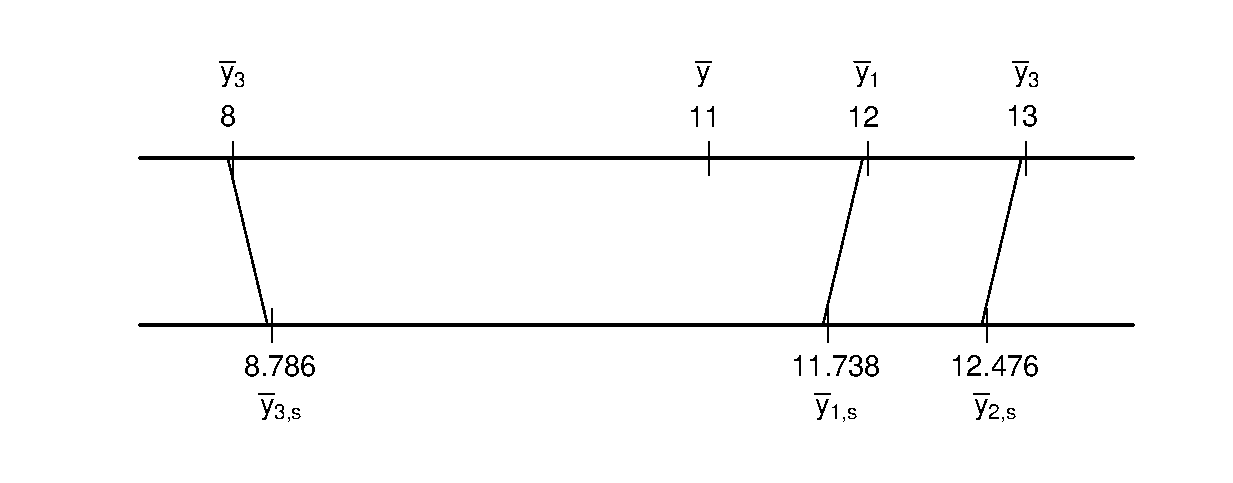
\includegraphics[width=1\textwidth]{Chapter18CredibilityBM/F18Shrinkage.eps}
    \caption{\label{F18:Shrinkage} \small  Comparison of Group-Specific Means to Shrinkage Estimates.
For an illustrative data set, group-specific and overall means are
graphed on the upper scale. The corresponding shrinkage estimates
are graphed on the lower scale. This figure shows the shrinkage
aspect of models with random effects. }
  \end{center}
\end{figure}

\linejed

Under the one-way random effects model, we have that $\bar{y}_i$ is
an unbiased predictor of $\mu+\alpha_i$ in the sense that E
($\bar{y}_i - (\mu+\alpha_i)$)=0. However, $\bar{y}_i$ is
inefficient in the sense that the shrinkage estimator,
$\bar{y}_{i,s}$, has a smaller mean square error than $\bar{y}_i$.
Intuitively, because $\bar{y}_{i,s}$  is a linear combination of
$\bar{y}_i$  and $\bar{y}$, we say that has been ``shrunk'' towards
the estimator $\bar{y}$. Further, because of the additional
information in $\bar{y}_{i,s}$, it is customary to interpret a
shrinkage estimator as ``borrowing strength'' from the estimator of
the overall mean.

Note that the shrinkage estimator reduces to the fixed effects
estimator $\bar{y}_i$  when the credibility factor, $\zeta$, becomes
1. It is easy to see that $\zeta \rightarrow 1$ as either (i)
$T\rightarrow\infty$ or (ii) $\sigma^2/\sigma^2_{\alpha}\rightarrow
0$. That is, the best predictor approaches the group mean as either
(i) the number of observations per group becomes large or (ii) the
variability among groups becomes large relative to the response
variability. In actuarial language, either case supports the idea
that the information from the $i$th group is becoming more
``credible.''

\subsection{Longitudinal Models}

As we have seen the context of the one-way random effects model with
balanced replications, B\"{u}hlmann's greatest accuracy credibility
estimator is equivalent to the best linear unbiased predictor
introduced in Section 15.1.3. This is also true when considering a
more general longitudinal sampling set-up introduced in Chapter 10
(see, for example, Frees, Young and Luo, 1999). By expressing the
credibility problem in terms of a regression-based sampling scheme,
we can use well-known regression techniques to estimate parameters
and predict unknown quantities. We now consider a longitudinal model
that handles many special cases of interest in actuarial practice.

Assume that claims experience follows
\begin{equation}\label{E18:MixedLinearModel}
y_{it} = M_i + \mathbf{x}_{it}^{\prime} \boldsymbol \beta+
\mathbf{z}_{it}^{\prime} {\boldsymbol \alpha}_i +
\varepsilon_{it},~~~~~ t=1, \ldots, T_i, i=1,\ldots, n.
\end{equation}\index{regression model!mixed linear}
Let us consider each model component in turn.
\begin{itemize}


\item $M_i$ represents the manual premium that is assumed known.
In the language of generalized linear models, $M_i$ is an ``offset
variable.'' In estimating the regression model, one simply uses
$y_{it}^{\ast} = y_{it} - M_i$ as the dependent variable. If the
manual premium is not available, then take $M_i = 0$.


\item $\mathbf{x}_{it}^{\prime} \boldsymbol \beta$ is the usual
linear combination of explanatory variables. These can be used to
adjust the manual premium. For example, you may have a larger than
typical proportions of males (or females) in your group and wish to
allow for the gender of group members. This can be done by using a
binary gender variable as a predictor and thinking of the regression
coefficient as the amount to adjust the manual premium. In a similar
fashion, you could use age, experience or other characteristics of
group members to adjust manual premiums. Explanatory variables may
also be used to describe the group, not just the members. For
example, you may wish to include explanatory variables that give
information about location of place of employment (such as urban
versus rural) to adjust manual premiums.

\item $\mathbf{z}_{it}^{\prime} {\boldsymbol \alpha}_i$ represents a
linear combination of random effects that can be written as
$\mathbf{z}_{it}^{\prime} {\boldsymbol \alpha}_i = z_{it,1}
\alpha_{i,1} + \cdots +z_{it,q} \alpha_{i,q}$. Often, there is only
a single random intercept so that $q=1$, $z_{it}=1$ and
$\mathbf{z}_{it}^{\prime} {\boldsymbol \alpha}_i = \alpha_{i1} =
\alpha_i$. The random effects have mean zero but a non-zero mean can
be incorporated using $\mathbf{x}_{it}^{\prime} \boldsymbol \beta$.
For example, we might use time $t$ as an explanatory variable and
define $\mathbf{x}_{it}=\mathbf{z}_{it}=(1 ~t)^{\prime}$. Then,
equation (\ref{E18:MixedLinearModel}) reduces to $y_{it} = \beta_0 +
\alpha_{i1} + ( \beta_1 + \alpha_{i2}) \times t+ \varepsilon_{it}$,
a model due to Hachemeister in 1975.

\item $\varepsilon_{it}$ is the mean zero disturbance term. In many
applications, a weight is attached to it in the sense that
$\mathrm{Var}~\varepsilon_{it} = \sigma^2 /w_{it}.$ Here, the weight
$w_{it}$ is known and accounts for an exposure such as the amount of
insurance premium, number of employees, size of the payroll, number
of insured vehicles and so forth. Introducing weights was proposed
by B\"{u}hlmann and Straub in 1970. The disturbances terms are
typically assumed independent among groups (over $i$) but, in some
applications, may incorporate time patterns, such as $AR$(1)
(autoregressive of order 1).

\end{itemize}



\linejed\empexjed{WorkersComp}\index{datasets!workers compensation}
\index{actuarial \& financial terms and concepts!workers
compensation}

\textbf{ Example: Workers Compensation.}\ecaptionjed{Workers
Compensation} We consider workers compensation insurance, examining
losses due to permanent, partial disability claims. The data are
from Klugman (1992), who explored Bayesian model representations,
and are originally from the National Council on Compensation
Insurance. We consider $n=121$ occupation classes over $T=7$ years.
To protect the data sources, further information on the occupation
classes and years are not available. We summarize the analysis in
Frees, Young and Luo (2001).

The response variable of interest is the pure premium (PP), defined
to be losses due to permanent, partial disability per dollar of
PAYROLL. The variable PP is of interest to actuaries because worker
compensation rates are determined and quoted per unit of payroll.
The exposure measure, PAYROLL, is one of the potential explanatory
variables. Other explanatory variables are YEAR (= 1, \ldots, 7) and
occupation class.

Among other representations, Frees et al. (2001) considered the
model B\"{u}hlmann-Straub model,
\begin{equation}\label{E18:WCBS}
\ln (PP)_{it} = \beta_0 + \alpha_{i1}+  \varepsilon_{it},
\end{equation}
the Hachemeister model
\begin{equation}\label{E18:WCHach}
\ln (PP)_{it} = \beta_0 + \alpha_{i1} + (\beta_1+\alpha_{i2})YEAR_t
+ \varepsilon_{it},
\end{equation}
and an intermediate version
\begin{equation}\label{E18:WCInt}
\ln (PP)_{it} = \beta_0 + \alpha_{i1}+  \alpha_{i2}YEAR_t +
\varepsilon_{it}.
\end{equation}
In all three cases, the weights given by $w_{it}= PAYROLL_{it}$.
These models are all special cases of the general model in equation
(\ref{E18:MixedLinearModel}) with $y_{it} = \ln (PP)_{it}$ and
$M_i=0$.

\linejed

Parameter estimation and related statistical inference, including
prediction, for the mixed linear regression model in equation
(\ref{E18:MixedLinearModel}) has been well investigated. The
literature is summarized briefly in Section 15.1. From Section
15.1.3, the best linear unbiased predictor of $\mathrm{E}(y_{it} |
\boldsymbol \alpha)$ is of the form
\begin{equation}\label{E18:MixedLinearModelBLUP}
M_i + \mathbf{x}_{it}^{\prime} \mathbf{b}_{GLS}+
\mathbf{z}_{it}^{\prime} \mathbf{a}_{BLUP,i},
\end{equation}
where $\mathbf{b}_{GLS}$ is the generalized least squares estimator
of $\boldsymbol \beta$ and the general expression for
$\mathbf{a}_{BLUP,i}$ is given in equation (15.11). This is a
general credibility estimator that can be readily calculated using
statistical packages.


\linejed

\textbf{Special Case: B\"{u}hlmann-Straub Model.} For the
B\"{u}hlmann-Straub model, the credibility factor is
\begin{equation*}
\zeta_{i,w} = \frac{WT_i}{WT_i + \sigma^2/\sigma^2_{\alpha}},
\end{equation*}
where $WT_i$ is the sum of weights for the $i$th group, $WT_i =
\sum_{t=1}^{T_i} w_{it}$.

Using equation (\ref{E18:MixedLinearModelBLUP}) in the
B\"{u}hlmann-Straub model, it is easy to check that the prediction
for the $i$th group is
\begin{equation*}
 \zeta_{i,w}  \bar{y}_{i,w} + (1-\zeta_{i,w} ) \bar{y}_w ,
\end{equation*}
where
\begin{equation*}
\bar{y}_{i,w} =\frac{\sum_{t=1}^{T_i} w_{it}y_{it}}{WT_i}
~~~~\mathrm{and}~~~~~~\bar{y}_w =\frac{\sum_{t=1}^{T_i} \zeta_{i,w}
\bar{y}_{i,w}}{\sum_{t=1}^{T_i} \zeta_{i,w} }
\end{equation*}
are the $i$th weighted group mean and the overall weighted mean,
respectively. This reduces to the balanced B\"{u}hlmann predictor by
taking weights identically equal to 1. See, for example, Frees
(2004, Section 4.7) for further details.





\linejed

\textbf{ Example: Workers Compensation - Continued.} We estimated
the models in equations (\ref{E18:WCBS})-(\ref{E18:WCInt}) as well
as the unweighted Buhlmann model using maximum likelihood. Table
\ref{T18:WorkersCompModelFits} summarizes the results. This table
suggest that the annual trend factor is not statistically
significant, at least for conditional means. The annual trend that
varies by occupational class does seem to be helpful. The
information criterion $AIC$ suggestions that the intermediate model
given in equation (\ref{E18:WCInt}) provides the best fit to the
data.

\begin{table}[h]
\scalefont{0.9} \caption{\label{T18:WorkersCompModelFits} Workers
Compensation Model Fits}
\begin{tabular}{lrrrr}\hline
    &   \multicolumn{2}{r}{B\"{u}hlmann-Straub} & Hachemeister \\
Parameter & B\"{u}hlmann & Eq (\ref{E18:WCBS}) &Eq (\ref{E18:WCHach}) & Eq (\ref{E18:WCInt}) \\
\hline
$\beta_0 $ & -4.3665 &  -4.4003&  -4.3805& -4.4036 \\
($t$-statistic) & (-50.38)& (-51.47) & (-44.38)& (-51.90) \\
$\beta_1 $    & & & -0.00446& \\
($t$-statistic) & & & (-0.47)  \\ \hline
$\sigma_{\alpha,1} $ &0.9106 &  0.8865 & 0.9634 & 0.9594\\
$\sigma_{\alpha,2} $ & &   & 0.0452 & 0.0446\\
$\sigma $ & 0.5871& 42.4379& 41.3386 & 41.3582\\\hline
$AIC $ & 1,715.924 & 1,571.391& 1,567.769&1,565.977 \\
\hline
\end{tabular}
\scalefont{1.1111}
\end{table}


Table \ref{T18:WorkersCompCredEstimates} illustrates the resulting
credibility predictions for the first five occupational classes.
Here, for each method, after making the prediction we exponentiated
the result and multiplied by 100, so that these are the number of
cents of predicted losses per dollar of payroll. Also included are
predictions for the ``fixed effects'' model that amount to taking
the average over occupational class for the seven year time span.
Predictions for the Hachemeister and equation (\ref{E18:WCInt})
models were made for Year 8.

Table \ref{T18:WorkersCompCredEstimates} shows substantial agreement
between the B\"{u}hlmann and B\"{u}hlmann-Straub predictions,
indicating that payroll weighting is less important for this data
set. There is also substantial agreement between the Hachemeister
and equation (\ref{E18:WCInt}) model predictions, indicating that
the overall time trend is less important. Comparing the two sets of
predictions indicates that a time trend that varies by occupational
class does make a difference.


\begin{table}[h]
\scalefont{0.9} \caption{\label{T18:WorkersCompCredEstimates}
Workers Compensation Predictions}
\begin{tabular}{crrrrr}\hline
Occupational & Fixed &             &B\"{u}hlmann-& &            Eq \\
Class   & Effects    & B\"{u}hlmann& Straub & Hachemeister  & (\ref{E18:WCInt}) \\
\hline \hline
         1 &      2.981 &      2.842 &      2.834 &      2.736 &      2.785 \\
         2 &      1.941 &      1.895 &      1.875 &      1.773 &      1.803 \\
         3 &      1.129 &      1.137 &      1.135 &      1.124 &      1.139 \\
         4 &      0.795 &      0.816 &      0.765 &      0.682 &      0.692 \\
         5 &      1.129 &      1.137 &      1.129 &      1.062 &      1.079 \\
\hline
\end{tabular}
\scalefont{1.1111}
\end{table}

\linejed

\section{Bonus-Malus}\label{S18:Bonus-Malus}\index{actuarial \& financial terms and concepts!bonus-malus}

Bonus-malus methods of experience rating are used extensively in
automobile insurance pricing in Europe and Asia. To understand this
type of experience rating, let us first consider pricing based on
observable characteristics. In automobile insurance, these include
driver characteristics (such as age and sex), vehicle
characteristics (such as car type and whether or not used for work)
and territory characteristics (such as county of residence). Use of
only these characteristics for pricing results in an \emph{a priori
premium}. In the US and Canada, this is the primary basis of the
premium; experience rating enters in a limited fashion in the form
of premium surcharges for at-fault accidents and moving traffic
violations.

Bonus-malus systems (BMS) provide a more detailed integration of
claims experience into the pricing. Typically, a BMS classifies
policyholders into one of several ordered categories. A policyholder
enters the system into a specific category. In the following year,
policyholders with an accident-free year are awarded a ``bonus'' and
moved up a category. Policyholders that experience at-fault
accidents during the year receive a ``malus'' and moved down a
specified number of categories. The category that one resides in
dictates the \textit{bonus-malus factor}, or \textit{BMF}. The
\emph{BMF} times the a priori premium is known as the \emph{a
posteriori premium}.\index{actuarial \& financial terms and
concepts!a posteriori premium}

To illustrate, Lemaire (1998) gives an example of a Brazilian system
that is summarized in Table \ref{T18:BrazilBMF}. In this system, one
begins in Class 7, paying 100\% of premiums dictated by the
insurer's a priori premium. In the following year, if the
policyholder experiences an accident-free year, he or she pays only
90\% of the a priori premium. Otherwise, the premium is 100\% of the
a priori premium.\index{actuarial \& financial terms and concepts!a
priori premium}

\begin{table}[h]\begin{center}
\scalefont{0.9} \caption{\label{T18:BrazilBMF} Brazilian Bonus-Malus
System}
\begin{tabular}{ccccccccc}
  \hline
   &  & \multicolumn{7}{c}{Class After}\\ \cline{3-9}\vspace{-.05in}\\
  Class  &      &  0 & 1 & 2 & 3 & 4 & 5 & $\geq 6$ \\
  Before & BMF & Claims & Claims & Claims & Claims & Claims & Claims & Claims \\  \hline
  7 & 100       & 6 & 7 & 7 & 7 & 7 & 7 & 7 \\
  6 & 90        & 5 & 7 & 7 & 7 & 7 & 7 & 7 \\
  5 & 85        & 4 & 6 & 7 & 7 & 7 & 7 & 7 \\
  4 & 80        & 3 & 5 & 6 & 7 & 7 & 7 & 7 \\
  3 & 75        & 2 & 4 & 5 & 6 & 7 & 7 & 7 \\
  2 & 70        & 1 & 3 & 4 & 5 & 6 & 7 & 7 \\
  1 & 65        & 1 & 2 & 3 & 4 & 5 & 6 & 7 \\
  \hline
   \multicolumn{9}{l}{\textit{Source}: Lemaire (1998)}
\end{tabular}\end{center}
\scalefont{1.1111}
\end{table}

As described in Lemaire (1998), the Brazilian system is simple
compared to others (the Belgian system has 23 classes). Insurers
operating in countries with detailed bonus-malus systems do not
require the extensive a priori rating variable compared to the US
and Canada. This typically means fewer underwriting expenses and
thus a less costly insurance system. Moreover, many argue that it is
fairer to policyholders in the sense that those with poor claims
experience bear the burden of higher premiums and one is not
penalized simply because of gender or other rating variables that
are outside of the policyholder's control. See Lemaire (1995) for a
broad discussion of institutional, regulatory and ethical issues
involving bonus-malus systems.


Throughout this book, we have seen how to use regression techniques
to compute a priori premiums. Dionne and C. Vanasse (1992) pointed
out the advantages of using a regression framework to calculate
bonus-malus factors. Essentially, they used latent variable to
represent a policyholder's unobserved tendencies to become involved
in an accident (aggressiveness, swiftness of reflexes) with
regression count models to compute a posterior premiums. See Denuit
et al. (2007) for a recent overview of this developing area.





\section{Further Reading and References}

See Norberg (1986) for an early account relating credibility theory
to the framework of mixed linear models. The treatment here follows
Frees, Young and Luo (1999).

By demonstrating that many important credibility models can be
viewed in a (linear) longitudinal data framework, we restrict our
consideration to certain types of credibility models. Specifically,
the longitudinal data models accommodate only unobserved risks that
are additive. This chapter does not address models of nonlinear
random effects that have been investigated in the actuarial
literature; see, for example, Taylor (1977) and Norberg (1980).
Taylor (1977) allowed insurance claims to be possibly infinite
dimensional using Hilbert space theory and established credibility
formulas in this general context. Norberg (1980) considered the more
concrete context, yet still general, of multivariate claims and
established the relationship between credibility and statistical
empirical Bayes estimation. As described in Section
\ref{S18:Bonus-Malus}, Denuit et al. (2007) provides a recent
overview of nonlinear longitudinal claim count models.

To account for the entire distribution of claims, a common approach
used in credibility is to adopt a Bayesian perspective. Keffer
(1929) initially suggested using a Bayesian perspective for
experience rating in the context of group life insurance.
Subsequently, Bailey (1945, 1950) showed how to derive the linear
credibility form from a Bayesian perspective as the mean of a
predictive distribution. Several authors have provided useful
extensions of this paradigm. Jewell (1980) extended Bailey's results
to a broader class of distributions, the exponential family, with
conjugate prior distributions for the structure variables.


\bigskip

\textbf{References}


\scalefont{0.9}

\begin{multicols}{2}


Bailey, Arthur (1945). A generalized theory of credibility.
\textit{Proceedings of the Casualty Actuarial Society} 32.

Bailey, Arthur (1950). Credibility procedures: LaPlace's
generalization of Bayes' rule and the combination of collateral
knowledge with observed data. \textit{Proceedings of the Casualty
Actuarial Society Society} 37, 7-23.

B\"{u}hlmann, Hans (1967). Experience rating and credibility.
\emph{ASTIN Bulletin} 4, 199-207.

B\"{u}hlmann, Hans and E. Straub (1970). Glaubw\"{u}rdigkeit f\"{u}r
schadens\"{a}tze. \emph{Mitteilungen der Vereinigung Schweizerischer
Versicherungs-Mathematiker} 70, 111-133.

Dionne, George and C. Vanasse (1992). Automobile insurance
ratemaking in the presence of asymmetrical information.
\textit{Journal of Applied Econometrics} 7, 149-165.

Denuit, Michel, Xavier Marechal, Sandra Pitrebois and Jean-Francois
Walhin (2007). \textit{Actuarial Modelling of Claim Counts: Risk
Classification, Credibility and Bonus-Malus Systems}. Wiley, New
York.

Frees, Edward W., Virginia R. Young, and Yu Luo (1999). A
longitudinal data analysis interpretation of credibility models.
\emph{Insurance: Mathematics and Economics} 24, 229-247.

Frees, Edward W., Virginia R. Young, and Yu Luo (2001). Case studies
using panel data models. \emph{North American Actuarial Journal}
5(4), 24-42.

Frees, Edward W. (2004). \textit{Longitudinal and Panel Data:
Analysis and Applications in the Social Sciences.} Cambridge
University Press, New York.

Hachemeister, Charles A. (1975). Credibility for regression models
with applications to trend. In \emph{Credibility: Theory and
Applications}, editor Paul M. Kahn. Academic Press, New York,
129-163.

Keffer, R (1929). An experience rating formula. \textit{Transactions
of the Actuarial Society of America} 30, 130-139.

Klugman, Stuart A. (1992). \emph{Bayesian Statistics in Actuarial
Science}. Kluwer, Boston.

Klugman, Stuart A, Harry H. Panjer and Gordon E. Willmot (2008).
\emph{Loss Models: From Data to Decisions}. John Wiley \& Sons,
Hoboken, New Jersey.

Lemaire, Jean (1995). \textit{Bonus-Malus Systems in Automobile
Insurance}. Kluwer, Boston.

Lemaire, Jean (1998). Bonus-malus systems: The European and Asian
approach to merit-rating. \emph{North American Actuarial Journal}
2(1), 26-47.

Mowbray, Albert H. (1914). How extensive a payroll exposure is
necessary to give a dependable pure premium. \textit{Proceedings of
the Casualty Actuarial Society} 1, 24-30.

Norberg, Ragnar (1980). Empirical Bayes credibility.
\textit{Scandinavian Actuarial Journal} 177-194.

Norberg, Ragnar (1986). Hierarchical credibility: Analysis of a
random effect linear model with nested classification.
\textit{Scandinavian Actuarial Journal} 204-22.

Taylor, Greg C. (1977). Abstract credibility. \textit{Scandinavian
Actuarial Journal} 149-68.

Whitney, Albert W. (1918). The theory of experience rating.
\textit{Proceedings of the Casualty Actuarial Society} 4.

\end{multicols}


\scalefont{1.1111}
